\documentclass{chi-ext}
% Please be sure that you have the dependencies (i.e., additional LaTeX packages) to compile this example.
% See http://personales.upv.es/luileito/chiext/

%% EXAMPLE BEGIN -- HOW TO OVERRIDE THE DEFAULT COPYRIGHT STRIP -- (July 22, 2013 - Paul Baumann)
% \copyrightinfo{Permission to make digital or hard copies of all or part of this work for personal or classroom use is granted without fee provided that copies are not made or distributed for profit or commercial advantage and that copies bear this notice and the full citation on the first page. Copyrights for components of this work owned by others than ACM must be honored. Abstracting with credit is permitted. To copy otherwise, or republish, to post on servers or to redistribute to lists, requires prior specific permission and/or a fee. Request permissions from permissions@acm.org. \\
% {\emph{CHI'14}}, April 26--May 1, 2014, Toronto, Canada. \\
% Copyright \copyright~2014 ACM ISBN/14/04...\$15.00. \\
% DOI string from ACM form confirmation}
%% EXAMPLE END -- HOW TO OVERRIDE THE DEFAULT COPYRIGHT STRIP -- (July 22, 2013 - Paul Baumann)

% Load basic packages
\usepackage{balance}  % to better equalize the last page
\usepackage{amssymb}  % mathematical symbols
\usepackage{graphics} % for EPS, load graphicx instead
\usepackage{pgfplots} % Bar charts
\usepackage{times}    % comment if you want LaTeX's default font
\usepackage{url}      % llt: nicely formatted URLs
\usepackage[utf8]{inputenc}
\usepackage{soul}
\sethlcolor{black}

\usepackage{tikz}
\usepackage{subcaption}

\title{Towards Touch-Based Medical Image Diagnosis Annotation}

\numberofauthors{6}
% Notice how author names are alternately typesetted to appear ordered in 2-column format;
% i.e., the first 4 autors on the first column and the other 4 auhors on the second column.
% Actually, it's up to you to strictly adhere to this author notation.
\author{
  \alignauthor{
  	\textbf{Francisco Maria Calisto}\\
  	\affaddr{Institute for Systems and Robotics (ISR/IST), LARSyS}\\
  	\affaddr{Instituto Superior T\'{e}cnico}\\
  	\affaddr{Universidade de Lisboa}\\
  	\email{francisco.calisto}
  }\alignauthor{
  	\textbf{Jacinto Carlos Nascimento}\\
  	\affaddr{Institute for Systems and Robotics (ISR/IST), LARSyS}\\
  	\affaddr{Instituto Superior T\'{e}cnico}\\
  	\affaddr{Universidade de Lisboa}\\
  	\email{jacinto.nascimento}
  }
  \vfil
  \alignauthor{
  	\textbf{Alfredo Ferreira}\\
  	\affaddr{INESC-ID}\\
  	\affaddr{Instituto Superior T\'{e}cnico}\\
  	\affaddr{Universidade de Lisboa}\\
  	\email{alfredo.ferreira}
  }\alignauthor{
  	\textbf{Daniel Gon\c{c}alves}\\
  	\affaddr{INESC-ID}\\
  	\affaddr{Instituto Superior T\'{e}cnico}\\
  	\affaddr{Universidade de Lisboa}\\
  	\email{daniel.j.goncalves}
  }
}

% Paper metadata (use plain text, for PDF inclusion and later re-using, if desired)
\def\plaintitle{Towards Touch-Based Medical Image Diagnosis Annotation}
\def\plainauthor{Francisco Maria Calisto}
\def\plainauthor{Jacinto Carlos Nascimento}
\def\plainauthor{Alfredo Ferreira}
\def\plainauthor{Daniel Gonçalves}
\def\plainkeywords{Touch-Based, Medical Image Diagnosis, Medical Visualization, Interaction Design, Human-Computer Interaction}
\def\plaingeneralterms{Documentation, Standardization}

\hypersetup{
  % Your metadata go here
  pdftitle={\plaintitle},
  pdfauthor={\plainauthor},  
  pdfkeywords={\plainkeywords},
  pdfsubject={\plaingeneralterms},
  % Quick access to color overriding:
  %citecolor=black,
  %linkcolor=black,
  %menucolor=black,
  %urlcolor=black,
}

\usepackage{graphicx}   % for EPS use the graphics package instead
\usepackage{balance}    % useful for balancing the last columns
\usepackage{bibspacing} % save vertical space in references


\begin{document}

\marginpar{
\begin{figure}
  \begin{center}
  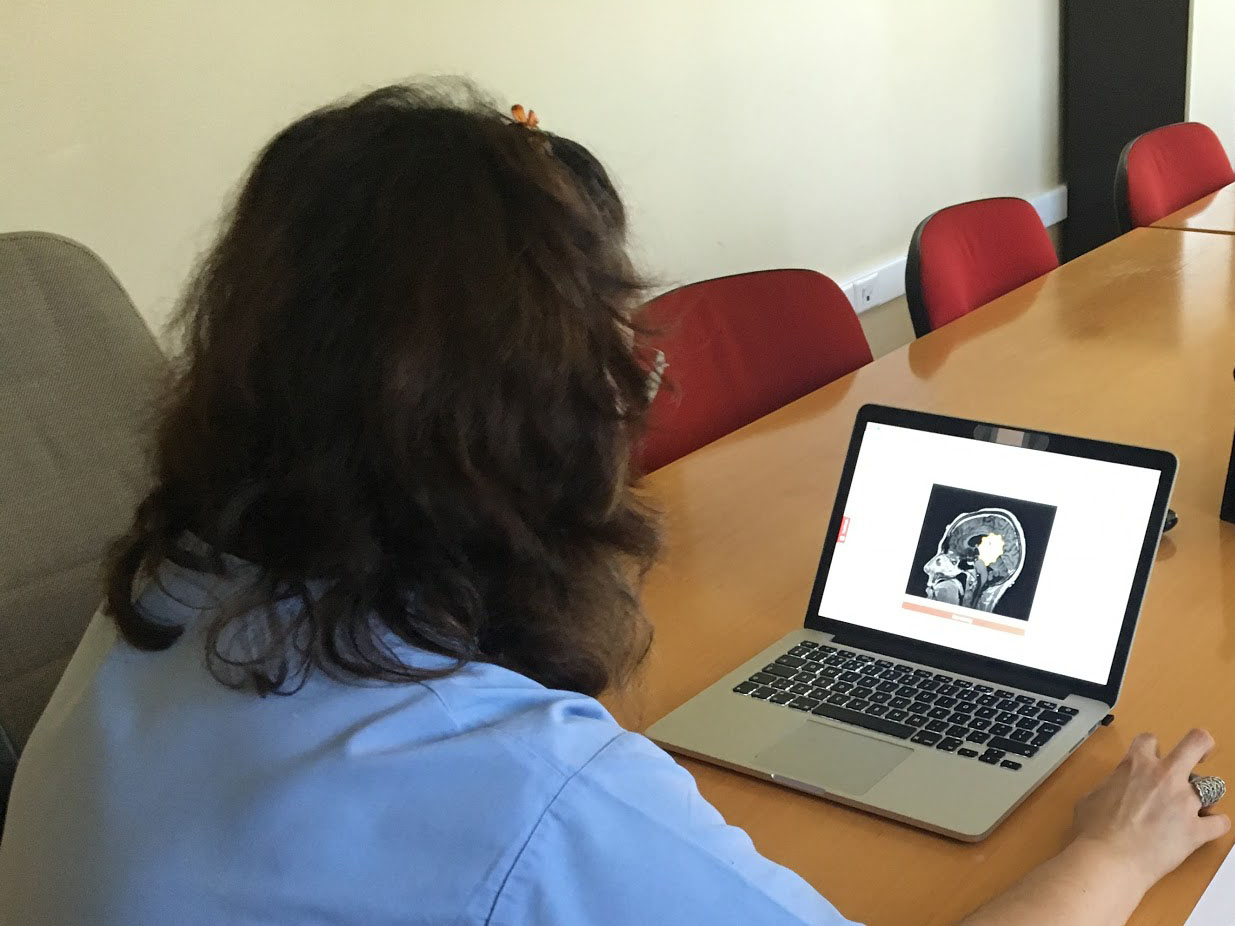
\includegraphics[width=\marginparwidth]{header_1.jpg}
  \caption{Radiologist interacting with traditional environment.}
  \label{fig:Fig1}
  \end{center}  
\end{figure}
}

\vfill

\marginpar{
\begin{figure}
  \begin{center}
  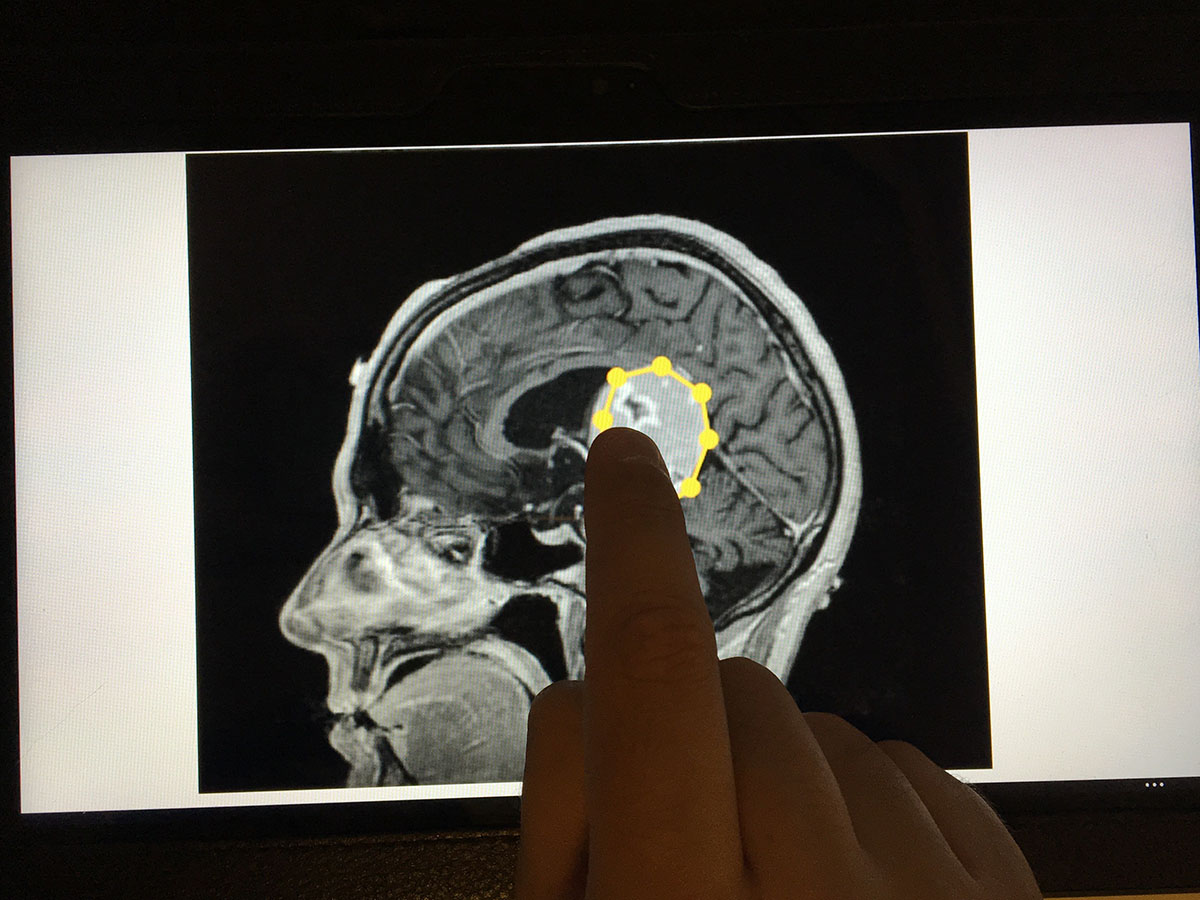
\includegraphics[width=\marginparwidth]{header_2.jpg}
  \caption{Touch environment interaction.}
  \label{fig:Fig2}
  \end{center}  
\end{figure}
}

\maketitle

\begin{abstract}

A fundamental step in medical diagnosis for patient follow-up relies on the ability of radiologists performing reliable diagnosis from acquired images. Basically, the diagnosis strongly depends on the visual inspection over the shape of the lesions, and somehow register its evolution through time. In existing clinical setups, a large number of images are currently acquired and should be individually inspected. As datasets increase in size, such visual evaluation becomes harder. For this reason it is crucial to introduce easy-to-use interfaces that help the radiologists not only to perform a reliable visual inspection but more importantly, allow the efficient delineation of the lesions. In this paper, we will present a study on integrating the above interfaces in a real-world scenario. More specifically, we will explore the radiologist's receptivity to the current touch environment solution. The advantages of touch are threefold: (i) the time performance is superior regarding the traditional use, (ii) it has more intuitive control and, (iii) for less time, the user interface delivers more information per action, concerning annotations. We concluded, from our studies that the path towards touch-based on medical image diagnosis annotation includes overcoming the current refusal to use these systems by radiologists, which resist change. Also, a solution to the finger occlusion must be devised.

\end{abstract}

\keywords{\plainkeywords}
\textcolor{red}{Optional section to be included in your final version.}

\category{H.5.m}{Information interfaces and presentation (e.g., HCI)}{Miscellaneous}. 
%See \cite{ACMCCS} 
See: \url{http://www.acm.org/about/class/1998/} 
for help using the ACM Classification system.
\textcolor{red}{Optional section to be included in your final version, but strongly encouraged.}


% =========================================================
\section{Introduction}
% =========================================================

\marginpar{
\begin{figure}
  \begin{center}
  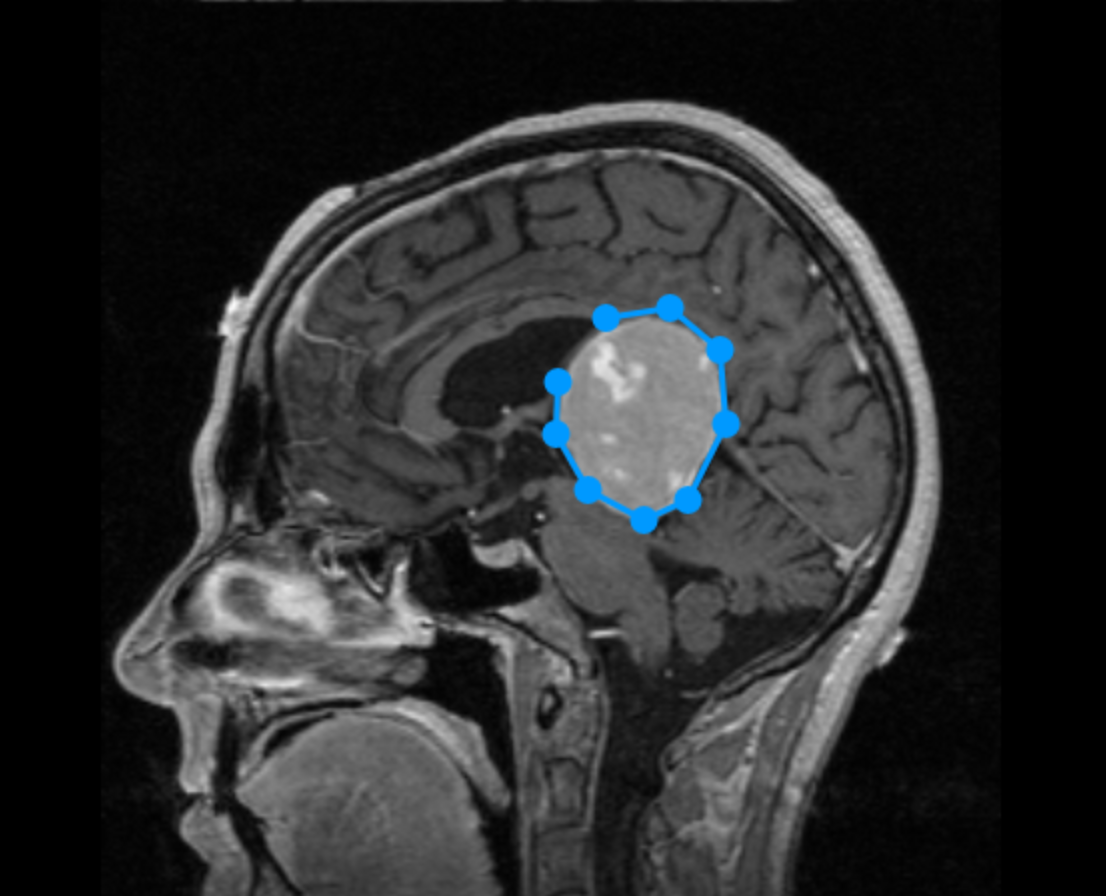
\includegraphics[width=\marginparwidth]{screen2.png}
  \caption{Hard difficulty DICOM annotated image.}
  \label{fig:Fig4}
  \end{center}  
\end{figure}
}
\marginpar{
\begin{figure}
  \begin{center}
  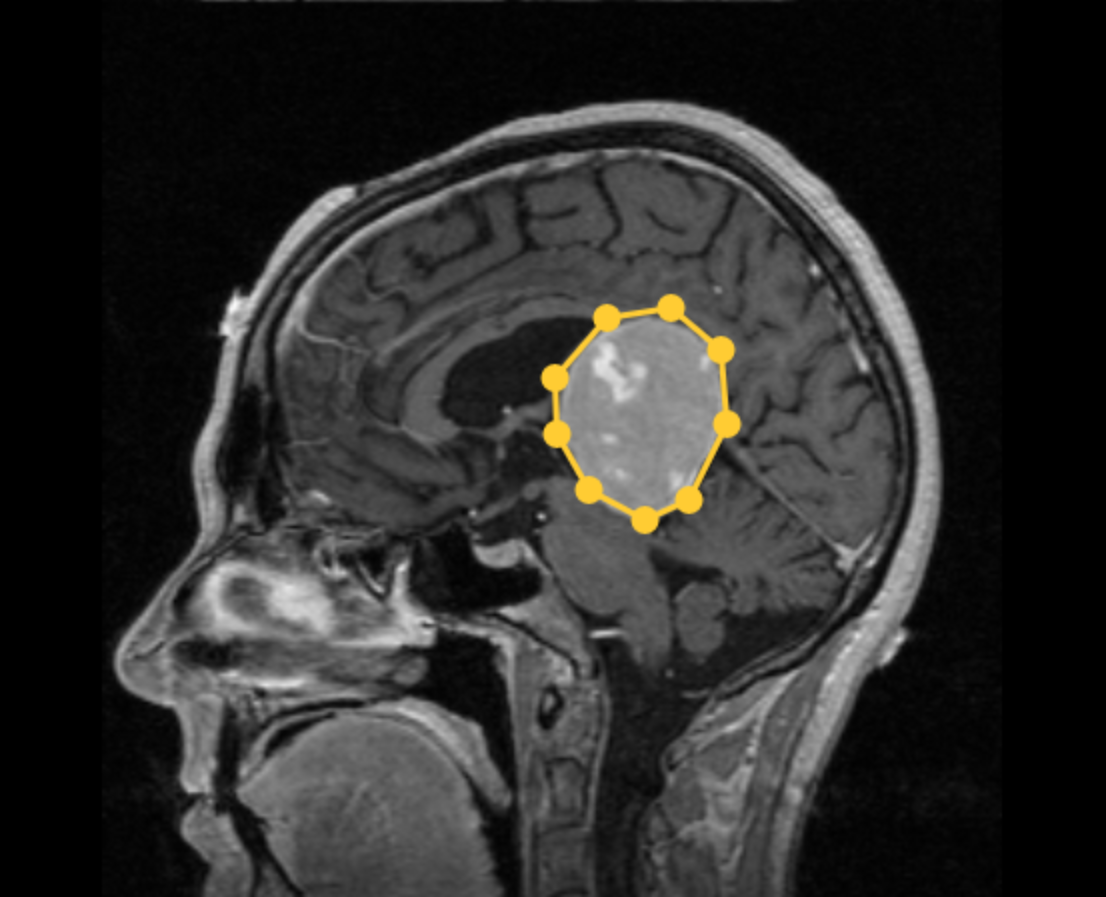
\includegraphics[width=\marginparwidth]{screen3.png}
  \caption{Hard difficulty DICOM annotated image.}
  \label{fig:Fig5}
  \end{center}  
\end{figure}
}
\marginpar{
\begin{figure}
  \begin{center}
  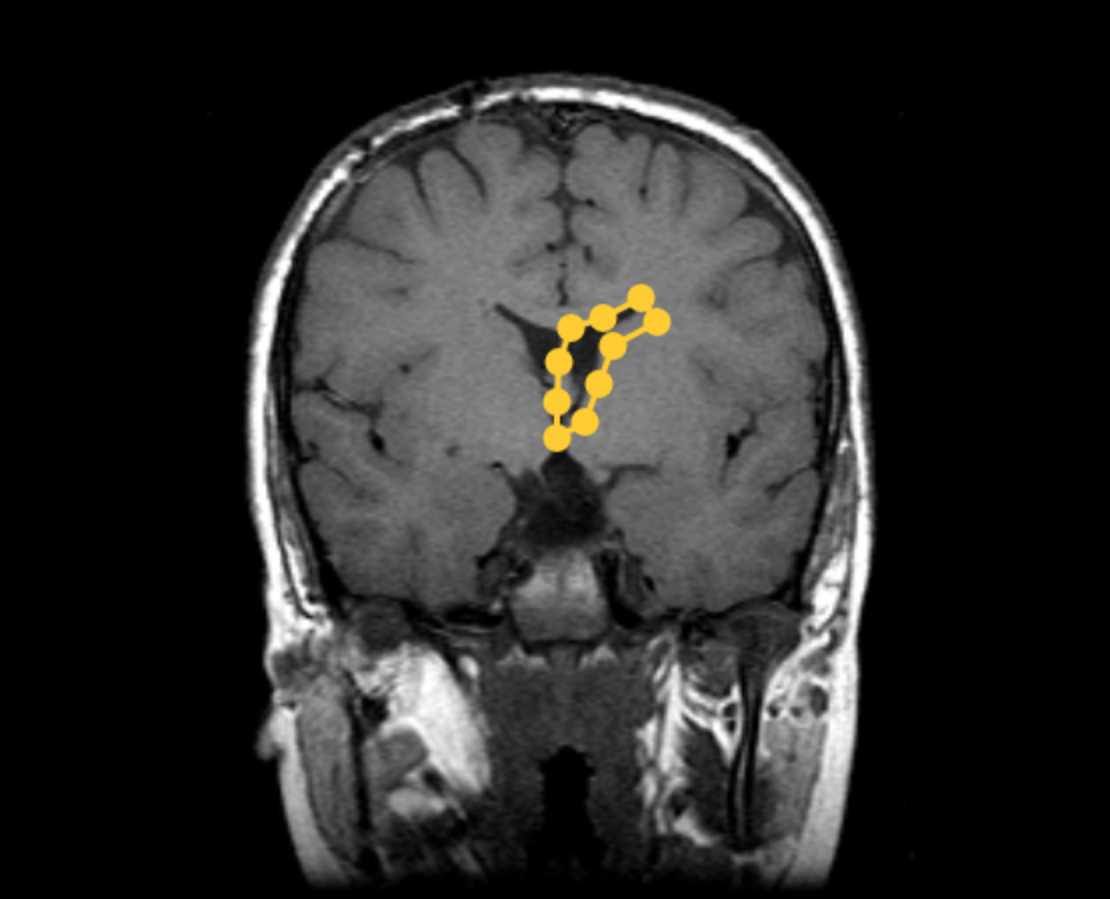
\includegraphics[width=\marginparwidth]{screen4.png}
  \caption{Hard difficulty DICOM annotated image.}
  \label{fig:Fig6}
  \end{center}  
\end{figure}
}

Medical imaging diagnosis is a topic of great interest, that has been the subject of intensive research in the field of medicine, and more specifically in Radiology~\cite{doi2007computer, seibel2005medical, doi2005current}. However, current tools do not fully support annotation collection. These annotations and their relationships are crucial for a proper diagnosis. Namely, to have the morphological time evolution of potential lesions that may be present in some organs.

In this paper, we present a performance and experience analysis conducting a study of touch and traditional environments (Figures \ref{fig:Fig1} and \ref{fig:Fig2}) that are aligned to the previous mentioned goals. Both environments are  comfortable to interact with and fast enough to solve the annotation tasks. For each environment, the same simple image feature (e.g. delete/correct annotation) is considered.

The performance differences of traditional and touch input devices have been studied~\cite{watson2013deconstructing} in terms of speed and accuracy for a variety of clinical and medical interactive tasks. This includes features such as Regions of Interest (ROI) annotations and length measurements, among others. Although, user experience while inserting annotations is important when evaluating the input devices, there is still a lack of research examining how the experience compromises the interactive surfaces based on the input type. To tackle this, our main goals focus primarily on cognition and time-performance. The experience is also considered as a means to validate the sensation, affect and value of  interaction.

Indeed, while user experience analysis and evaluation has been applied to clinical systems~\cite{crisan2013optimization},  time-measure and error scales are still missing. Moreover, a touch interactive surface application can improve medical and clinical competences, since it is able to reduce the running time figures to complete common tasks in the diagnosis loop.

\section{Evaluation}

Table \ref{tab:Tab1} shows the order of the user (radiologist) tests. It can be seen that the ``Order 1'' column is the opposite regarding the ``Order 2'' column. In the ``Order 1'' column, the user trains on the mouse-based environment, then executes a set of pre-defined tasks, followed by a questionnaire. This procedure is then repeated for the touch environment. In the ``order 2'' column is similar, with the users training and performing their tasks in the touch setting first. Half of the users first perform the mouse and keyboard test, and the other half perform first the touch tests.

\subsection{Task}

Radiologists interact with this user interface by doing some annotations on some regions of interest areas. The images are chosen to be representative to the domain field and to understand the different levels of the difficulty in these images. In our work, the first task is to perform the annotations on the DICOM Image 1 along with the brain lesion near of the cortex as we can see on Figure \ref{fig:Fig4} and Figure \ref{fig:Fig5}. The second image is almost similar of the first one (just a different frame) so the task was the same. The last image we put radiologists doing some more difficult annotation as it is shown in Figure \ref{fig:Fig6}.

\marginpar{
\begin{table}
  \centering
  \def\arraystretch{1.5}
  \begin{tabular}{|c|c|c|}
    \hline
    \tabhead{Phase} &
    \multicolumn{1}{|p{0.15\columnwidth}|}{\centering\tabhead{Order 1}} &
    \multicolumn{1}{|p{0.15\columnwidth}|}{\centering\tabhead{Order 2}} \\
    \hline
    1 & Tr (M) & Tr (T) \\
    \hline
    2 & M & T \\
    \hline
    3 & Q (M) & Q (T) \\
    \hline
    4 & Tr (T) & Tr (M) \\
    \hline
    5 & T & M \\
    \hline
    6 & Q (T) & Q (M) \\
    \hline
    7 & QF & QF \\
    \hline
  \end{tabular}
  \caption{Study Ordering. Both Conditions (M = Mouse, T = Touch) took 5 minutes. Training (Tr) and Quiz (Q) took less then 1 minute. Participants complete a final questionnaire (QF = Final Quiz) that took less then 5 minutes.}
  \label{tab:Tab1}
\end{table}
}

\subsection{Measures}

The following scales are considered: (i) Starting by the Positive and Negative Affect Scale~\cite{watson1999panas} (PANAS), (ii) Intrinsic Motivation Inventory~\cite{ryan1982control} (IMI) and (iii), Experience Needs Satisfaction~\cite{broeck2010capturing} (ENS). When we achieve the end of the condition, radiologists are asked to provide information and rank each condition, providing any comments.

\subsubsection{Performance}

We measure accuracy by computing the Hit Rate Score (HRS). This measure is defined has the percentage of annotations that lie on three areas (Figure \ref{fig:Fig7}). These three areas are measured from the ground-truth (see black line in Figure \ref{fig:Fig7}). The first area, \textbf{Area A}, is the area delimited by the two \textbf{Green Lines}, having a width of $2\epsilon$, where $\epsilon$ is the perpendicular distance from a point in the ground truth (black line) to the \textbf{Green Line}\footnote{Here, the $\epsilon$ is the diameter of the annotation point.}. The second area, \textbf{Area B}, has also a width of $2\epsilon$. However,  \textbf{Area B} embraces two regions, each region falling between the \textbf{Green Lines} (inner boundary) and \textbf{Red Lines} (outer boundary).

\subsubsection{User Experience}

To evaluate the user experience we embed, the IMI~\cite{ryan1982control}, PANAS~\cite{watson1999panas}
and ENS~\cite{broeck2010capturing} measures in a 5-point Likert-scales,  ranging from 1 (strongly disagree) to 5 (strongly agree).

\section{Results}

Since the data collected does not meet the applicability pre-conditions required for ANOVA, i.e., does not follow a Gaussian distributions and also the number of samles is small, we resort to use the Kruskal-Wallis Analysis of Variance~\cite{theodorsson1986kruskal} to test the performance and experience that is useful for testing between-subjects effects for three or more conditions~\cite{mcfarlane2002comparison}.

Figure \ref{fig:Fig8}  gives the overall results of the Kruskal-Wallis test. This result shows that all the mean differences for each of the radiologists is significant in the above 13 conditions.

\begin{figure}
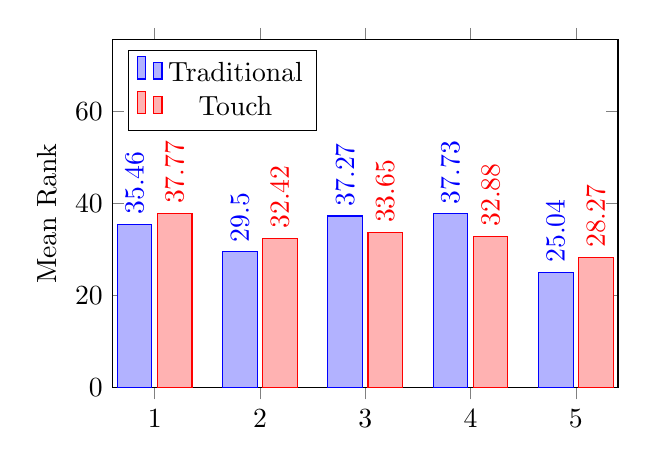
\begin{tikzpicture}
    \begin{axis}[
        ybar,
        every node near coord/.append style={rotate=90, anchor=west},
        ymin=0,
        width  = 8cm,
        height = 6cm,
        bar width=12.50pt,
        ylabel={Mean Rank},
        nodes near coords,
        xticklabel style={rotate=0},
        xtick = data,
        table/header=false,
        table/row sep=\\,
        xticklabels from table={
          1\\2\\3\\4\\5\\
          }{[index]0},
        enlarge y limits={value=1.00,upper},
        legend pos=north west
    ]
    \addplot table[x expr=\coordindex,y index=0]{35.46\\29.50\\37.27\\37.73\\25.04\\};
    \addplot table[x expr=\coordindex,y index=0]{37.77\\32.42\\33.65\\32.88\\28.27\\};
    \legend{Traditional, Touch}
    \end{axis}
\end{tikzpicture}
\caption{Kruskal-Wallis.}
\label{fig:Fig8}
\end{figure}

A small number of radiologists is used in the tests. Three of the five radiologists (1, 2 and 5) have shown that touch environment is better classified then traditional environment. Although, we must consider and understand the other two radiologist (3 and 4) results. The Kruskal-Wallis test\footnote{
\textit{env}: environment (\textit{env}) with both traditional (\textit{tra}) and touch (\textit{tou}) options;

$\chi^2\textsubscript{env}$: Chi-Square of the environment (\textit{env});

$\alpha\textsubscript{env}$: Alpha value of the environment (\textit{env});
} revealed that radiologists have a significant main effect on touch environment ($\chi^2\textsubscript{tou} = 1.711$, $\alpha\textsubscript{tou} = 0.789$), against traditional environment ($\chi^2\textsubscript{tra} = 4.587$, $\alpha\textsubscript{tra} = 0.332$).

In the following sections (Figure \ref{fig:Fig8} - Figure \ref{fig:Fig12}) we describe the results in terms of the first and second order statistics, using the mean ($M\textsubscript{env}$) and standard deviation ($\sigma\textsubscript{env}$), as well as the standard error of the mean\footnote{
\textit{N}: the number of users (radiologists);

$sem\textsubscript{env}$: standard error of the mean for the environment (\textit{env});

$M\textsubscript{env}$: mean value of the environment \textit{env};

$\sigma\textsubscript{env}$: standard deviation of the environment \textit{env};
} that is defined as:

\begin{center}
$sem\textsubscript{env} = \sigma\textsubscript{env}/\sqrt{N}$
\end{center}

\subsection{Performance}

\marginpar{
\begin{figure}
  \begin{center}
  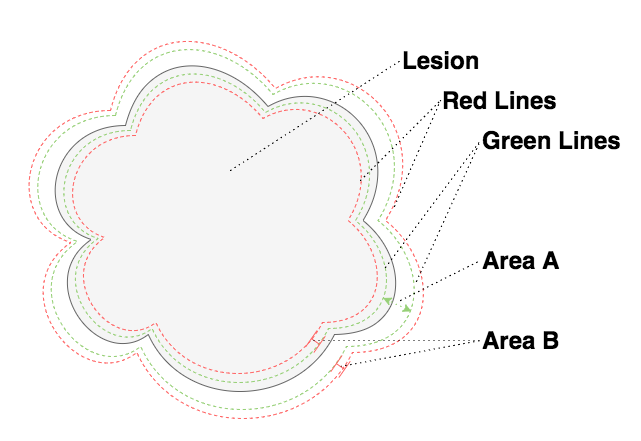
\includegraphics[width=\marginparwidth]{mimbcd-ui_areas.png}
  \caption{Annotation Classification Areas.}
  \label{fig:Fig7}
  \end{center}
\end{figure}
}

Figure \ref{fig:Fig9} shows the mean time performance of the tasks as described in Section task.

\textit{Time}. A significant main effect of the traditional input environment (M\textsubscript{tra}=153.4s, $\sigma$\textsubscript{tra}=40.88, {\mathop{\rm sem\textsubscript{tra}}}$\left({\bar x}\right)=18.28$) with radiologist maximum time spent of 210 seconds and radiologist minimum time spent of 109 seconds. For the touch input environment (M\textsubscript{tou}=114.20s, $\sigma$\textsubscript{tou}=51.71, {\mathop{\rm sem\textsubscript{tou}}}$\left({\bar x}\right)=23.12$) the radiologists take less time, however the standard error ({\mathop{\rm sem\textsubscript{tou}}}$\left({\bar x}\right)=23.12$) is higher on touch input environment.
  
\textit{Number of Interactions (NI)}.  There is a main effect on input of the total number of interactions (M\textsubscript{tra}=39.20, $\sigma$\textsubscript{tra}=4.65, {\mathop{\rm sem\textsubscript{tra}}}$\left({\bar x}\right)=2.08$), where the mean of the interactions on traditional (M\textsubscript{tra}=39.20) is less  (M\textsubscript{tou}=40) than the touch environment.

\textit{Hit Rate Score (HRS)}. It is shown that the HRS, where the traditional environment (M\textsubscript{tra}=75.2, $\sigma$\textsubscript{tra}=22.72, {\mathop{\rm sem\textsubscript{tra}}}$\left({\bar x}\right)=10.16$), has a higher value then touch environment (M\textsubscript{tou}=50.6, $\sigma$\textsubscript{tou}=15.35, {\mathop{\rm sem\textsubscript{tou}}}$\left({\bar x}\right)=6.86$).

\subsection{User Experience}

Responses to the final questionnaire suggest that both interactions are adequate for analyzing medical images. Moreover no radiologist reported discomfort, dizziness or fatigue in neither environment.

\subsubsection{Motivational}

The motivational results are presented as \textit{Competence}, \textit{Autonomy}, \textit{Relatedness} and \textit{Immersion} (Figure \ref{fig:Fig10}) options.

\begin{figure}
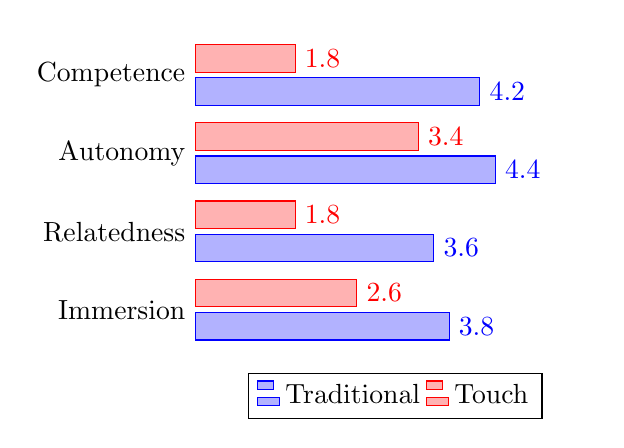
\begin{tikzpicture}
\begin{axis}[
align = center,
xbar,
y axis line style = { opacity = 0 },
axis x line       = none,
tickwidth         = 0pt,
height = 5.75cm,
enlarge y limits  = 0.20,
enlarge x limits  = 0.50,
symbolic y coords = {Immersion, Relatedness, Autonomy, Competence},
legend style={at={(0.5,-0.05)},
    anchor=north,legend columns=-1},
nodes near coords,
]
\addplot coordinates {
% TRADITIONAL
(3.8,Immersion)
(3.6,Relatedness)
(4.4,Autonomy)
(4.2,Competence)

};
\addplot coordinates {
% TOUCH
(2.6,Immersion)
(1.8,Relatedness)
(3.4,Autonomy)
(1.8,Competence)

};
\legend{Traditional, Touch}
\end{axis}
\end{tikzpicture}
\caption{Motivation Experience}
\label{fig:Fig10}
\end{figure}

\textit{Competence}. The main outcome on traditional environment (M\textsubscript{tra}=4.2, $\sigma$\textsubscript{tra}=0.83, {\mathop{\rm sem\textsubscript{tra}}}$\left({\bar x}\right)=0.37$), showed that radiologists feel more comfortable in traditional environment, as it can be expected. On the other hand, for touch environment (M\textsubscript{tou}=3.4, $\sigma$\textsubscript{tou}=1.67, {\mathop{\rm sem\textsubscript{tou}}}$\left({\bar x}\right)=0.74$), radiologists showed a rated above average, however, lower than traditional environment.

\marginpar{
\begin{figure}
\centering 

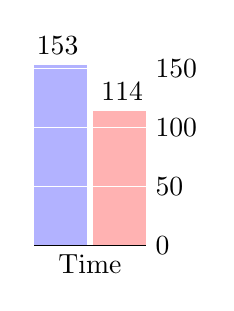
\begin{tikzpicture}
\begin{axis}[
    ybar, axis on top,
    height=4cm, width=3cm,
    bar width=0.75cm,
    ymajorgrids, tick align=inside,
    major grid style={draw=white},
    enlarge y limits={value=0.01,upper},
    ymin=0, ymax=160,
    axis x line*=bottom,
    axis y line*=right,
    y axis line style={opacity=0},
    tickwidth=0pt,
    enlarge x limits=true,
    legend style={
        at={(0.5,-0.2)},
        anchor=north,
        legend columns=-1,
        /tikz/every even column/.append style={column sep=0.5cm}
    },
    %ylabel={Seconds (s)},
    symbolic x coords={
       Time},
   xtick=data,
   nodes near coords={
    \pgfmathprintnumber[precision=0]{\pgfplotspointmeta}
   }
]
% TRADITIONAL
\addplot [draw=none, fill=blue!30] coordinates {
  (Time,153.40) };
% TOUCH
\addplot [draw=none,fill=red!30] coordinates {
  (Time,114.20) };

\end{axis}
\end{tikzpicture}% NO EMPTY LINE HERE!!!! 
\begin{tikzpicture}
\begin{axis}[
    ybar, axis on top,
    height=4cm, width=3cm,
    bar width=0.75cm,
    ymajorgrids, tick align=inside,
    major grid style={draw=white},
    enlarge y limits={value=0.01,upper},
    ymin=0, ymax=50,
    axis x line*=bottom,
    axis y line*=right,
    y axis line style={opacity=0},
    tickwidth=0pt,
    enlarge x limits=true,
    legend style={
        at={(0.5,-0.2)},
        anchor=north,
        legend columns=-1,
        /tikz/every even column/.append style={column sep=0.5cm}
    },
    %ylabel={Mean},
    symbolic x coords={
       NI},
   xtick=data,
   nodes near coords={
    \pgfmathprintnumber[precision=0]{\pgfplotspointmeta}
   }
]
% TRADITIONAL
\addplot [draw=none, fill=blue!30] coordinates {
  (Performance Time,39.20) };
% TOUCH
\addplot [draw=none,fill=red!30] coordinates {
  (Performance Time,40.00) };

\end{axis}
\end{tikzpicture}
\begin{tikzpicture}
\centering
\begin{axis}[
    ybar, axis on top,
    height=4cm, width=3cm,
    bar width=0.75cm,
    ymajorgrids, tick align=inside,
    major grid style={draw=white},
    enlarge y limits={value=0.01,upper},
    ymin=0, ymax=80,
    axis x line*=bottom,
    axis y line*=right,
    y axis line style={opacity=0},
    tickwidth=0pt,
    enlarge x limits=true,
    legend style={
        at={(0.5,-0.2)},
        anchor=north,
        legend columns=-1,
        /tikz/every even column/.append style={column sep=0.5cm}
    },
    %ylabel={Score},
    symbolic x coords={
       HRS},
   xtick=data,
   nodes near coords={
    \pgfmathprintnumber[precision=0]{\pgfplotspointmeta}
   }
]
% TRADITIONAL
\addplot [draw=none, fill=blue!30] coordinates {
  (Hit Rate,75.20) };
% TOUCH
\addplot [draw=none,fill=red!30] coordinates {
  (Hit Rate,50.60) };

\end{axis}
\end{tikzpicture}
\caption{Time Performance Mean; Number of Interactions (NI) Mean; Hit Rate Score (HRS) Mean.} \label{fig:Fig9}
\end{figure}
}

\textit{Autonomy}. The traditional environment reflected (M\textsubscript{tra}=4.4, $\sigma$\textsubscript{tra}=0.89, {\mathop{\rm sem\textsubscript{tra}}}$\left({\bar x}\right)=0.4$) a high average level of autonomy with three radiologists choosing a $\max_{}$(x\textsubscript{tra}) = 5. For the touch environment we also have values above average (M\textsubscript{tou}=3.4, $\sigma$\textsubscript{tou}=1.14, {\mathop{\rm sem\textsubscript{tou}}}$\left({\bar x}\right)=0.5$), we also have a $\max_{}$(x\textsubscript{tou}) = 5 but just one radiologist scored this value.

\textit{Relatedness}. Radiologists relatedness show us a touch environment below the average (M\textsubscript{tou}=1.8, $\sigma$\textsubscript{tou}=0.44, {\mathop{\rm sem\textsubscript{tou}}}$\left({\bar x}\right)=0.2$), where the $\max_{}$(x\textsubscript{tou}) = 2 and the $\min_{}$(x\textsubscript{tou}) = 1.  On the other hand, the traditional environment (M\textsubscript{tra}=3.6, $\sigma$\textsubscript{tra}=1.14, {\mathop{\rm sem\textsubscript{tra}}}$\left({\bar x}\right)=0.5$), we have the mean (M\textsubscript{tra}=3.6) above average, and the rest values typically normal. The $\max_{}$(x\textsubscript{tou}) = 5 and the $\min_{}$(x\textsubscript{tou}) = 2.

\textit{Immersion}. For motivational experience, the immersion values of traditional environment (M\textsubscript{tra}=3.8, $\sigma$\textsubscript{tra}=1.3, {\mathop{\rm sem\textsubscript{tra}}}$\left({\bar x}\right)=0.58$) are above average at the mean value (M\textsubscript{tra}=3.8). We have here a $\max_{}$(x\textsubscript{tra}) = 5 and the $\min_{}$(x\textsubscript{tra}) = 2, however two radiologists voted x\textsubscript{tra} = 5 the mean value (M\textsubscript{tra}=3.8) was not that high. The touch environment provided (M\textsubscript{tou}=2.6, $\sigma$\textsubscript{tou}=1.51, {\mathop{\rm sem\textsubscript{tou}}}$\left({\bar x}\right)=0.67$).

\subsubsection{Pleasure and Enjoyment}

We present the results of \textit{Affect}, \textit{Enjoyment} and \textit{Intuitive Controls} (Figure \ref{fig:Fig11}).

\begin{figure}
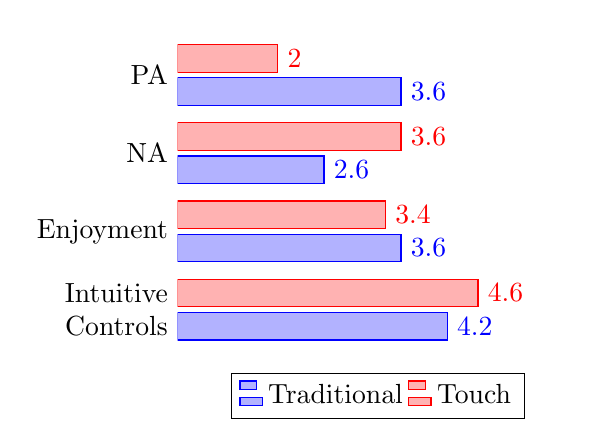
\begin{tikzpicture}
\begin{axis}[
align = center,
xbar,
y axis line style = { opacity = 0 },
axis x line       = none,
tickwidth         = 0pt,
height = 5.75cm,
enlarge y limits  = 0.20,
enlarge x limits  = 0.50,
symbolic y coords = {Intuitive\\Controls, Enjoyment, NA, PA},
legend style={at={(0.5,-0.05)},
    anchor=north,legend columns=-1},
nodes near coords,
]
\addplot coordinates {
% TRADITIONAL
(3.6,PA)
(2.6,NA)
(3.6,Enjoyment)
(4.2,Intuitive\\Controls)

};
\addplot coordinates {
% TOUCH
(2,PA)
(3.6,NA)
(3.4,Enjoyment)
(4.6,Intuitive\\Controls)

};
\legend{Traditional, Touch}
\end{axis}
\end{tikzpicture}
\caption{Overall Pleasure and Enjoyment of the Task}
\label{fig:Fig11}
\end{figure}

\textit{Affect}. The rise of the field of affective computing has placed an emphasis on understanding the affective and cognitive-affective responses that radiologists have to their technological interactions. Traditional environment is perceived as more positive (M\textsubscript{tra}=3.6, $\sigma$\textsubscript{tra}=0.54, {\mathop{\rm sem\textsubscript{tra}}}$\left({\bar x}\right)=0.24$), whereas the marginal negative affect for traditional environment (M\textsubscript{tra}=2.6, $\sigma$\textsubscript{tra}=0.54, {\mathop{\rm sem\textsubscript{tra}}}$\left({\bar x}\right)=0.24$) showed a typical correlation. The touch environment is perceived as more negative (M\textsubscript{tou}=2, $\sigma$\textsubscript{tou}=0.7, {\mathop{\rm sem\textsubscript{tou}}}$\left({\bar x}\right)=0.31$) then positive (M\textsubscript{tou}=3.6, $\sigma$\textsubscript{tou}=1.14, {\mathop{\rm sem\textsubscript{tou}}}$\left({\bar x}\right)=0.5$).

\textit{Enjoyment}. Intrinsic motivation is foundations of the enjoyment of interactive experiences, and can be attributed to volition and achievement inherent in the person. The traditional environment provides (M\textsubscript{tra}=3.6, $\sigma$\textsubscript{tra}=1.14, {\mathop{\rm sem\textsubscript{tra}}}$\left({\bar x}\right)=0.51$) which is almost the same as in the touch environment (M\textsubscript{tou}=3.4, $\sigma$\textsubscript{tou}=1.67, {\mathop{\rm sem\textsubscript{tou}}}$\left({\bar x}\right)=0.74$).

\clearpage
 
\textit{Intuitive Controls}. Controls are intuitive when they do not interfere with one's sense of presence being easily mastered. For the intuitive controls the overall system was high rated by radiologists, however the behavior of traditional environment (M\textsubscript{tra}=4.2, $\sigma$\textsubscript{tra}=0.44, {\mathop{\rm sem\textsubscript{tra}}}$\left({\bar x}\right)=0.2$) was less 8\% than touch environment (M\textsubscript{tou}=4.6, $\sigma$\textsubscript{tou}=0.54, {\mathop{\rm sem\textsubscript{tou}}}$\left({\bar x}\right)=0.24$).

\section{Acknowledgments}

I would like to convey our gratefulness to Hospital Fernando Fonseca (HFF) for the collaboration. I would specially like to thank the Doctors Clara Aleluia, Gisela Andrade, Willian Schmitt and Ana Sofia Germano from the HFF for the generous support and medical expertise. My appreciation goes also to Bruno Cardoso and Bruno Dias for help and above all for the good companionship. Thanks to Professors Daniel Sim\~{o}es Lopes and Daniel Mendes for the support. Last but not least, thank to Joana Teixeira and L\'{i}dia Freitas for the feedback. This work was partially supported by Funda\c{c}\~{a}o para a Ci\^{e}ncia e a Tecnologia (FCT) and Instituto Superior T\'{e}cnico (IST) through the RD0461-LARSys-ISR-CC930403:UID/EEA/50009/2013 project, BL89/2017-IST-ID grant.

\balance
\bibliographystyle{acm-sigchi}
\bibliography{sample}

\end{document}